% ============================================================================
%  Mid-semester BTP presentation -- 8 slides, paced for a 5-minute video
%
%  OVERLEAF SETUP
%    1. Same project as the report, or a new one -- paste as slides.tex
%    2. The figures/ folder must contain the five PDFs from
%       evaluation/results/figures/
%    3. Compile with pdfLaTeX
%
%  The speaking script is in report/presentation_script.md, with timings
%  that match these slides one-to-one.
% ============================================================================
\documentclass[aspectratio=169,10pt]{beamer}

\usetheme{default}
\usecolortheme{seagull}
\usepackage{graphicx}
\usepackage{booktabs}
\usepackage{appendixnumberbeamer}

\setbeamertemplate{navigation symbols}{}
\setbeamertemplate{footline}[frame number]
\setbeamerfont{frametitle}{size=\large,series=\bfseries}
\setbeamercolor{frametitle}{fg=black}
\setbeamertemplate{itemize item}{\textbullet}
\setlength{\parskip}{4pt}

% One accent, used only for the number that matters on each slide.
\definecolor{hl}{HTML}{B8442A}
\definecolor{ok}{HTML}{2A5751}
\newcommand{\hl}[1]{\textcolor{hl}{\textbf{#1}}}
\newcommand{\ok}[1]{\textcolor{ok}{\textbf{#1}}}

\title{\textbf{A Multi-Agent System for Time-Series\\Modelling across Domains}}
\subtitle{Mid-semester: the framework, and its first capability validated}
\author{Kaveri Neeli}
\institute{\small Indian Institute of Technology Indore}
\date{\small Mid-semester review}

\begin{document}

% ---------------------------------------------------------------- 1 (0:00)
\begin{frame}[plain]
  \titlepage
\end{frame}

% ---------------------------------------------------------------- 2 (0:20)
\begin{frame}{The goal, and what is delivered this semester}
  \begin{columns}[T]
    \begin{column}{0.52\textwidth}
Time-series questions come in kinds: forecast a value, detect an anomaly,
      estimate an event probability, assess risk. Each needs a different model,
      and the right one also depends on the domain.

      \vspace{0.6em}
      \textbf{Goal:} \hl{one agent that decides which analysis to run}, choosing
      on measured evidence rather than a language model's judgement.

      \vspace{0.6em}
      \textbf{This semester:} the framework (20 models, 10 tasks, 4 domains),
      plus \ok{one task taken end to end} on two domains.
    \end{column}
    \begin{column}{0.44\textwidth}
      \small
      \textbf{Why anomaly detection first}
      \vspace{0.4em}

      It is the hardest of the four to evaluate honestly, so it tests the
      framework's weakest point.

      \vspace{0.5em}
      And it inverts between domains: a transit \textbf{repeats}, a crash
      happens \textbf{once}. If selection copes with that, the design
      generalises.
    \end{column}
  \end{columns}
\end{frame}

% ---------------------------------------------------------------- 3 (0:55)
\begin{frame}{The agent}
  \centering
  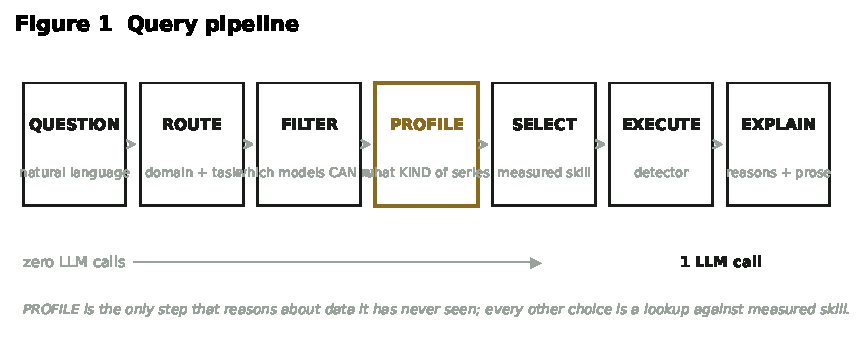
\includegraphics[width=0.97\textwidth]{figures/fig_pipeline.pdf}

  \vspace{0.6em}
  \begin{columns}[T]
    \begin{column}{0.48\textwidth}
      \small
      Every choice is made from a \textbf{registry of measured skill} ---
      20 models, each declaring what it needs, what it returns, and how well
      it actually scored.
    \end{column}
    \begin{column}{0.48\textwidth}
      \small
      \ok{PROFILE} is the one step that reasons about data it has never seen:
      it measures periodicity and decides whether events \emph{repeat} or
      happen \emph{once}.
    \end{column}
  \end{columns}
\end{frame}

% ---------------------------------------------------------------- 4 (1:35)
\begin{frame}{Selection: measured skill beats asking a language model}
  \begin{columns}[T]
    \begin{column}{0.54\textwidth}
      \centering
      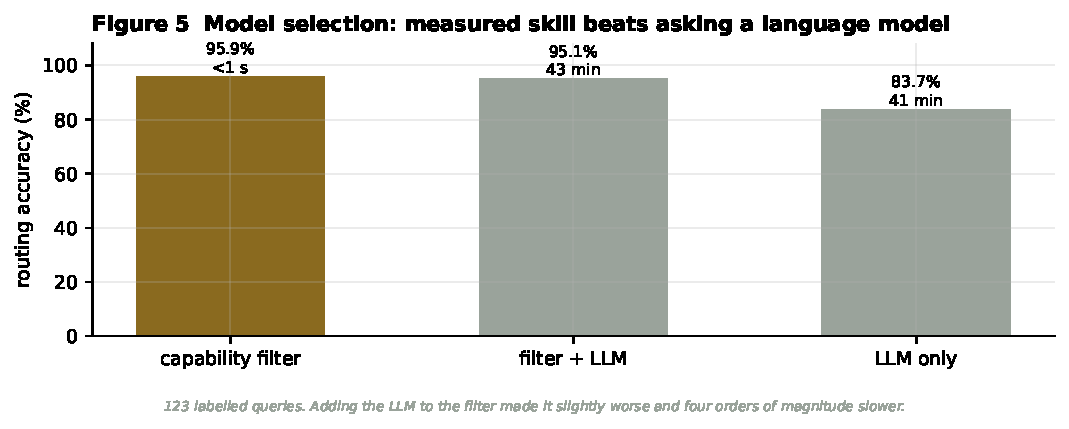
\includegraphics[width=\textwidth]{figures/fig_routing.pdf}
    \end{column}
    \begin{column}{0.42\textwidth}
      \small
      123 labelled queries: canonical phrasings, paraphrases, adversarial
      cases, and questions no model can answer.

      \vspace{0.8em}
      \begin{tabular}{@{}lrr@{}}
        \toprule
        & accuracy & time \\
        \midrule
        Capability filter & \ok{95.9\%} & $<$1 s \\
        LLM only          & 83.7\%      & 41 min \\
        Both              & 95.1\%      & 41 min \\
        \bottomrule
      \end{tabular}

      \vspace{0.8em}
      Adding the language model made it \hl{worse}.
    \end{column}
  \end{columns}
\end{frame}

% ---------------------------------------------------------------- 5 (2:15)
\begin{frame}{Getting the experiment right}
  \begin{columns}[T]
    \begin{column}{0.48\textwidth}
      \textbf{Labels must not come from the series being scored}

      \vspace{0.4em}
      \small
      An earlier version labelled a window ``transit'' by thresholding its own
      \emph{depth}, then tested detectors that look for deep dips.
      Measured inflation: \hl{+0.11 AUC}.

      \vspace{0.6em}
      Now: NASA ephemerides ($T_0 + nP$) for astronomy, a pre-registered event
      calendar for finance.

      \vspace{0.6em}
      Solar is excluded --- a flare's class is \emph{defined} by an X-ray
      threshold, so detecting flares from X-ray flux cannot fail.
    \end{column}
    \begin{column}{0.48\textwidth}
      \textbf{And the data has to be audited}

      \vspace{0.4em}
      \small
      Wu \& Keogh's four flaws, run on my own datasets \emph{before} any
      result was recorded:

      \vspace{0.5em}
      \begin{tabular}{@{}lcc@{}}
        \toprule
        & Kepler & Equity \\
        \midrule
        Triviality        & pass & pass \\
        Anomaly density   & \hl{warn} & pass \\
        Run-to-failure    & pass & pass \\
        Label quality     & pass & pass \\
        \bottomrule
      \end{tabular}

      \vspace{0.6em}
      No point adjustment: under it, a \emph{random} score reaches
      state-of-the-art $F_1$.
    \end{column}
  \end{columns}
\end{frame}

% ---------------------------------------------------------------- 6 (3:00)
\begin{frame}{The main result: nothing clears the floor}
  \centering
  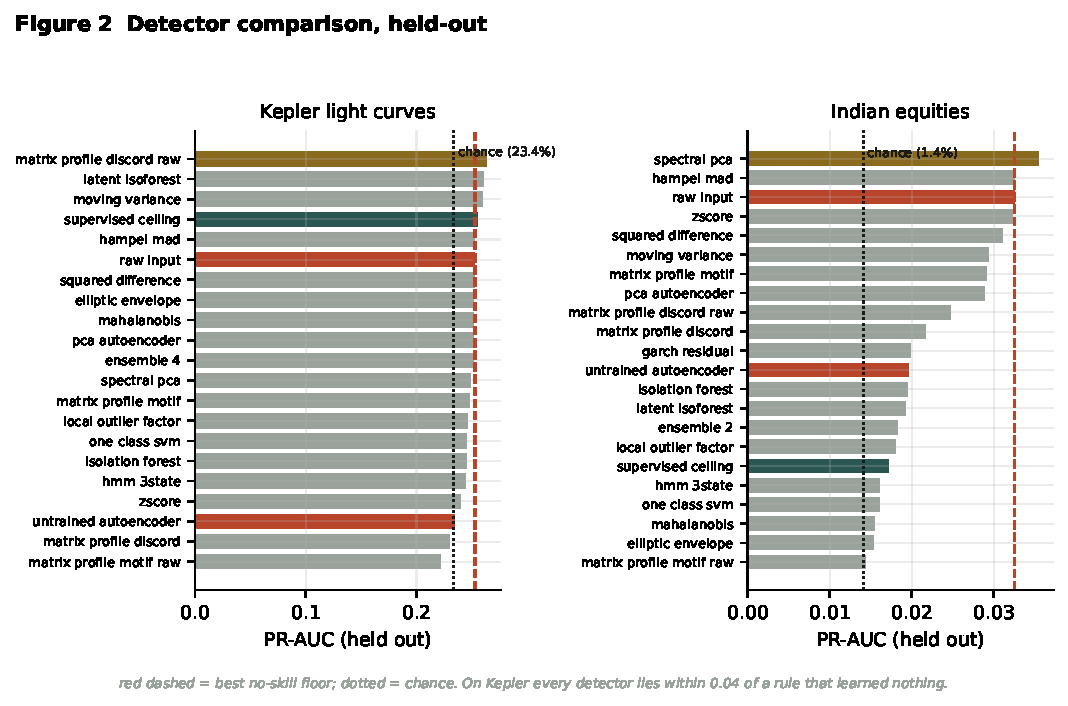
\includegraphics[height=0.62\textheight]{figures/fig_grid.pdf}

  \vspace{0.4em}
  \small
  22 detectors --- thresholds, isolation forest, one-class SVM, autoencoders,
  LSTM, matrix profile --- on two unrelated domains, scored \textbf{held out}.

  On Kepler the best beats a rule that learned nothing by \hl{0.0102 PR-AUC},
  and a supervised model \emph{given the labels} is outscored by three
  unsupervised ones.
\end{frame}

% ---------------------------------------------------------------- 7 (3:40)
\begin{frame}{Why in-sample scores lie}
  \begin{columns}[T]
    \begin{column}{0.56\textwidth}
      \centering
      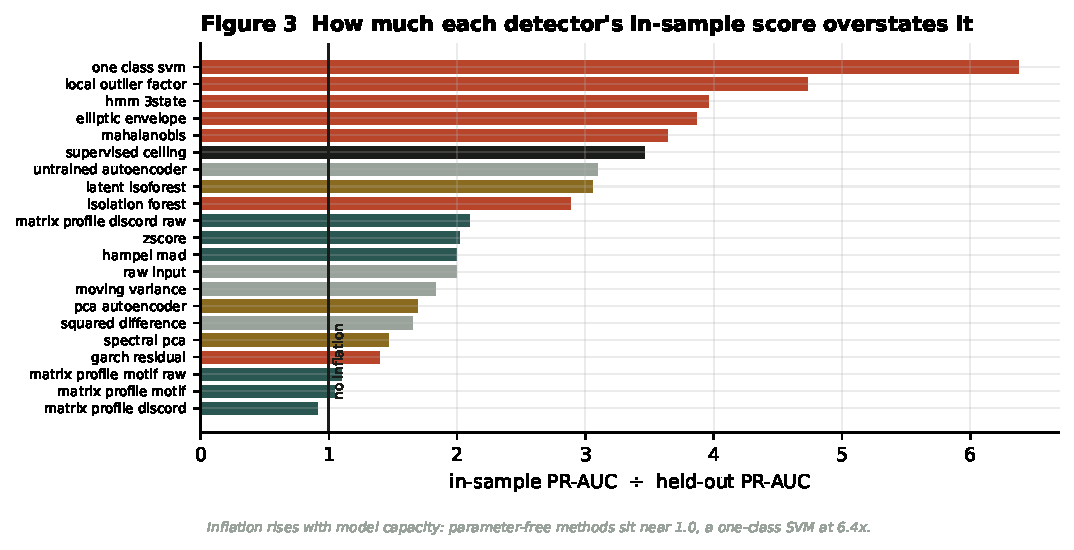
\includegraphics[width=\textwidth]{figures/fig_inflation.pdf}
    \end{column}
    \begin{column}{0.40\textwidth}
      \small
      Inflation $=$ in-sample $\div$ held-out.

      \vspace{0.6em}
      \begin{tabular}{@{}lr@{}}
        \toprule
        matrix profile    & 1.0$\times$ \\
        threshold rules   & 2.0$\times$ \\
        isolation forest  & 2.9$\times$ \\
        local outlier factor & 4.7$\times$ \\
        one-class SVM     & \hl{6.4$\times$} \\
        \bottomrule
      \end{tabular}

      \vspace{0.8em}
      It rises with \textbf{capacity}, not skill.

      \vspace{0.5em}
      Transductively the one-class SVM looked like the best equity detector
      at 4.62$\times$ lift. Held out: \hl{1.14$\times$}.
    \end{column}
  \end{columns}
\end{frame}

% ---------------------------------------------------------------- 8 (4:15)
\begin{frame}{The limit is the representation, not the algorithm}
  \begin{columns}[T]
    \begin{column}{0.54\textwidth}
      \centering
      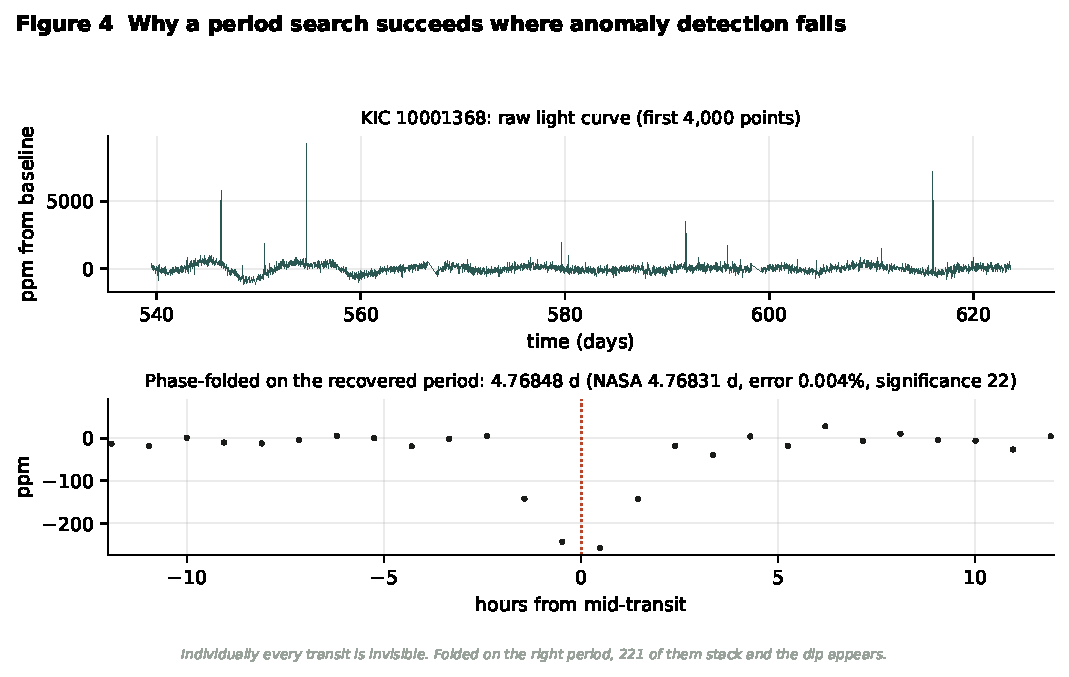
\includegraphics[width=\textwidth]{figures/fig_transit.pdf}
    \end{column}
    \begin{column}{0.42\textwidth}
      \small
      A transit recurs \textbf{221 times} --- so it is the \emph{least}
      unusual feature of its own light curve. Generic anomaly detection
      searches for the opposite of what is there.

      \vspace{0.6em}
      Change the question. Box Least Squares folds on thousands of candidate
      periods and stacks every repetition:

      \vspace{0.5em}
      \begin{tabular}{@{}lr@{}}
        \toprule
        significant peak & 91.4\% \\
        period within 1\% & \ok{60.9\%} \\
        median period error & 0.005\% \\
        \bottomrule
      \end{tabular}

      \vspace{0.5em}
      Across all \textbf{440} targets.
    \end{column}
  \end{columns}
\end{frame}

% ---------------------------------------------------------------- 9 (4:45)
\begin{frame}{Where this goes}
  \begin{columns}[T]
    \begin{column}{0.48\textwidth}
      \textbf{Delivered}
      \vspace{0.4em}
      \small
      \begin{itemize}
        \item The framework: 20 models, 10 tasks, 4 domains, selection on
              measured skill
        \item Selection beats an LLM by 12 points and costs nothing
        \item First task validated end to end: 22 detectors, two domains,
              none clears a no-skill floor
        \item In-sample advantage scales with capacity, not skill
      \end{itemize}
    \end{column}
    \begin{column}{0.48\textwidth}
      \textbf{Second half: the remaining tasks}
      \vspace{0.4em}
      \small
      \begin{itemize}
        \item \textbf{Risk:} regime-conditional Value-at-Risk, which passes the
              coverage tests the unconditional version fails
        \item \textbf{Forecasting:} bring those models to the same held-out
              standard and register their skill
        \item \textbf{Third domain:} Fermi blazar light curves, which the
              profiler predicts behave like equities, not Kepler
        \item \textbf{Ablation:} bare LLM vs.\ retrieval vs.\ full agent
      \end{itemize}
    \end{column}
  \end{columns}
\end{frame}

\appendix
\begin{frame}[plain]
  \centering
  \vspace{2em}
  {\Large \textbf{Thank you}}

  \vspace{1em}
  \small Kaveri Neeli \textbar{} \texttt{ep230051010@iiti.ac.in}
\end{frame}

\end{document}
